\documentclass[9pt]{beamer}
\usepackage{ctex, hyperref}
\usepackage[T1]{fontenc}

% \usepackage[orientation=landscape,size=custom,width=16,height=9,scale=0.4,debug]{beamerposter}
% 修改 slides 比例, 

% other packages
\usepackage{latexsym,amsmath,amssymb,amsthm,xcolor,multicol,booktabs,calligra}
\usepackage{graphicx,pstricks,listings,stackengine,cite}
\usepackage{subfigure}
\usepackage{tikz}
\usetikzlibrary{positioning, shapes.geometric}

\setbeamertemplate{bibliography item}[text]
\bibliographystyle{plain}
% 如果参考文献太多的话, 可以像下面这样调整字体:
% \tiny\bibliographystyle{plain}

\title{Solving Stiff ODEs}
% \subtitle{毕业设计答辩}
\institute{Department of Mathematics, Zhejiang University.}
\date{June 6th, 2023.}
\usepackage{College}

% defs
\def\cmd#1{\texttt{\color{red}\footnotesize $\backslash$#1}}
\def\env#1{\texttt{\color{blue}\footnotesize #1}}
\definecolor{deepblue}{rgb}{0,0,0.5}
\definecolor{deepred}{rgb}{0.6,0,0}
\definecolor{deepgreen}{rgb}{0,0.5,0}
\definecolor{halfgray}{gray}{0.55}

\lstset{
    basicstyle=\ttfamily\small,
    keywordstyle=\bfseries\color{deepblue},
    emphstyle=\ttfamily\color{deepred},    % Custom highlighting style
    stringstyle=\color{deepgreen},
    numbers=left,
    numberstyle=\small\color{halfgray},
    rulesepcolor=\color{red!20!green!20!blue!20},
    frame=shadowbox,
}


\begin{document}

\author{Wenchong Huang}

\kaishu
\begin{frame}
    \titlepage
    \begin{figure}[htpb]
        \begin{center}
            \vspace*{-0.5cm}
            \includegraphics[width=0.2\linewidth]{pic/zju.jpg}
        \end{center}
    \end{figure}
\end{frame}

\begin{frame}
    \tableofcontents[sectionstyle=show,subsectionstyle=show/shaded/hide,subsubsectionstyle=show/shaded/hide]
\end{frame}

\section{An overview}

\begin{frame}
  \frametitle{An overview of all methods}
\begin{table}[H]
  \centering
  \tiny
  \renewcommand\arraystretch{1.1}
  \begin{tabular}{cccc|cc|ccc}
  Method          & Abbreviation         & Approch                  &  Step Size         & Stages & Order  & A-Stable & B-Stable & L-Stable  \\ \hline
  Classical RK  & CLRK           & Explicit                  &  Constant        &  $4$   &  $4$    &      &      &            \\
  ESDIRK  & ESDIRK & Implicit  &  Constant        &  $6$   &  $4$    &   Yes   &   Yes   &    Yes   \\
  Gauss-Legendre  & GLRK$s$          & Implicit              &  Constant         &  $s$   &  $2s$    &   Yes   &   Yes   &      \\
  Radau-IIA  & RIIARK$s$             & Implicit              &  Constant         &  $s$   &  $2s-1$    &   Yes   &  Yes   &   Yes   \\
  Fehlberg  &  FB4(5)      & Explicit    &  Adaptive       &  $6$   & $4$  &        &      &         \\
  Dormand-Prince  &  DOPRI5   & Explicit       &  Adaptive       &  $7$   & $5$  &        &      &     \\    
  Dormand-Prince 8(7)  &  DOPRI8     & Explicit     &  Adaptive       &  $13$   & $8$  &        &      &     \\    
  Adaptive ESDIRK  & A-ESDIRK & Implicit  &  Adaptive       &  $6$   &  $4$    &   Yes   &   Yes   &    Yes   \\
  Adaptive Gauss-Legendre & A-GLRK$s$  & Implicit                       &  Adaptive         &  $s$   &  $2s$    &   Yes   &   Yes   &      \\
  Adaptive Radau-IIA & A-RIIARK$s$     & Implicit                       &  Adaptive         &  $s$   &  $2s-1$    &   Yes   &  Yes   &   Yes   
  \end{tabular}
\end{table}
\end{frame}

\section{An implemention of implicit RK methods}

\begin{frame}
  \frametitle{A simple iterative method}

  As known to us, we cannot compute $\mathbf{y}_i$ directly in implicit RK methods. For the ESDIRK method, we have
  \begin{equation*}
    \mathbf{y}_i=\mathbf{f}(\mathbf{z}_i+\gamma \mathbf{y}_i,t_n+c_ik),
  \end{equation*}
  where $\mathbf{z}_i$ is a konwn vector. We can set $\mathbf{y}_i\gets\mathbf{f}(\mathbf{U}^n,t_n)$ initially. Then update $\mathbf{y}_i$ for several times by the above equation. And we can compute $\mathbf{y}_1,...,\mathbf{y}_4$ in order.

  For collocation methods, we have
  \begin{equation*}
    \mathbf{y}_i=\mathbf{f}\left(\mathbf{U}^n+k\sum_{j=1}^s a_{ij} \mathbf{y}_j,t_n+c_ik\right),\quad i=1,...,s.
  \end{equation*}
  We can set $\mathbf{y}_i\gets\mathbf{f}(\mathbf{U}^n,t_n)\;(i=1,...,s)$ initially. Then update $\mathbf{y}_1,...,\mathbf{y}_s$ in order for several times.

  \textbf{Remark.} In the case that $\mathbf{f}(\mathbf{U},t)=A\mathbf{U}+\mathbf{b}(t)$, the $\mathbf{y}_i$s can be computed directly by solving the linear systems. Suppose $\mathbf{U}^n$ is a vector of dimension $m$. The ESDIRK method needs to solve an $m\times m$ system for $s$ times, while the collocation methods need to solve an $sm\times sm$ system for one time. The ESDIRK method will be much faster.
\end{frame}

\begin{frame}
  \frametitle{The Newton method}
  Sometimes the simple iterative method mentioned above does not work. So we need another method. Rewrite
  \begin{equation*}
    \mathbf{y}_i=\mathbf{f}\left(\mathbf{U}^n+k\sum_{j=1}^s a_{ij} \mathbf{y}_j,t_n+c_ik\right),\quad i=1,...,s
  \end{equation*}
  as
  \begin{equation*}
    \mathbf{F}(\mathbf{p})=\mathbf{0}, \quad \text{where} \quad \mathbf{p}=(\mathbf{y}_1^T,...,\mathbf{y}_s^T)^T.
  \end{equation*}

  The Newton method gives that
  \begin{equation*}
    \mathbf{p}\gets \mathbf{p}-J(\mathbf{F}(\mathbf{p}))^{-1}\mathbf{F}(\mathbf{p}),
  \end{equation*}
  where $J$ is the Jacobi matrix. To get the jacobi matrix, the derivatives should be computed. If someone uses
  \begin{equation*}
    g'(x)\approx \frac{g(x+h)-g(x-h)}{2h}
  \end{equation*}
  to compute the numerical derivative, then $h$ should be carefully chosen. The best choice is
  \begin{equation*}
    h=\sqrt[3]{\frac{3\mathbf{\epsilon}}{M}}.
  \end{equation*}
  where $\mathbf{\epsilon}$ is the machine precision and $M=\sup |g'''(x)|$.
\end{frame}

\section{An introduction to stiff equations}

\begin{frame}
  \frametitle{Definition}
  A \textbf{stiff equation} is a differential equation for which certain numerical methods for solving the equation are numerically unstable, unless the step size is taken to be extremely small.\footnote{From Wikipedia.}

  \vspace{1em}
  \textbf{Stiff equations} are equations where certain implicit methods, in particular BDF, perform better, usually tremendously better, than explicit ones.\footnote{Form Curtiss and Hirschfelder.}

  \vspace{1em}
  \textbf{Stiff equations} are problems for which explicit methods don't work.\footnote{From Hairer.}

  \vspace{1em}
  An IVP is said to be \textbf{stiff in an interval} if for some initial condition any numerical method with a bounded RAS is forced to use a time-step size that is unneccesarily and excessively smaller than the time scale of the true solution of the IVP.\footnote{From the textbook.}
\end{frame}

\begin{frame}
  \frametitle{A sample stiff problem}
  The IVP in Example 11.144
  \begin{equation}
    u'(t)=\lambda(u-\cos t)-\sin t,\quad u(0)=\eta,
  \end{equation}
  where $\lambda=-10^6$ and $\eta=1.5$ is a stiff problem.

  \begin{figure}
    \centering
    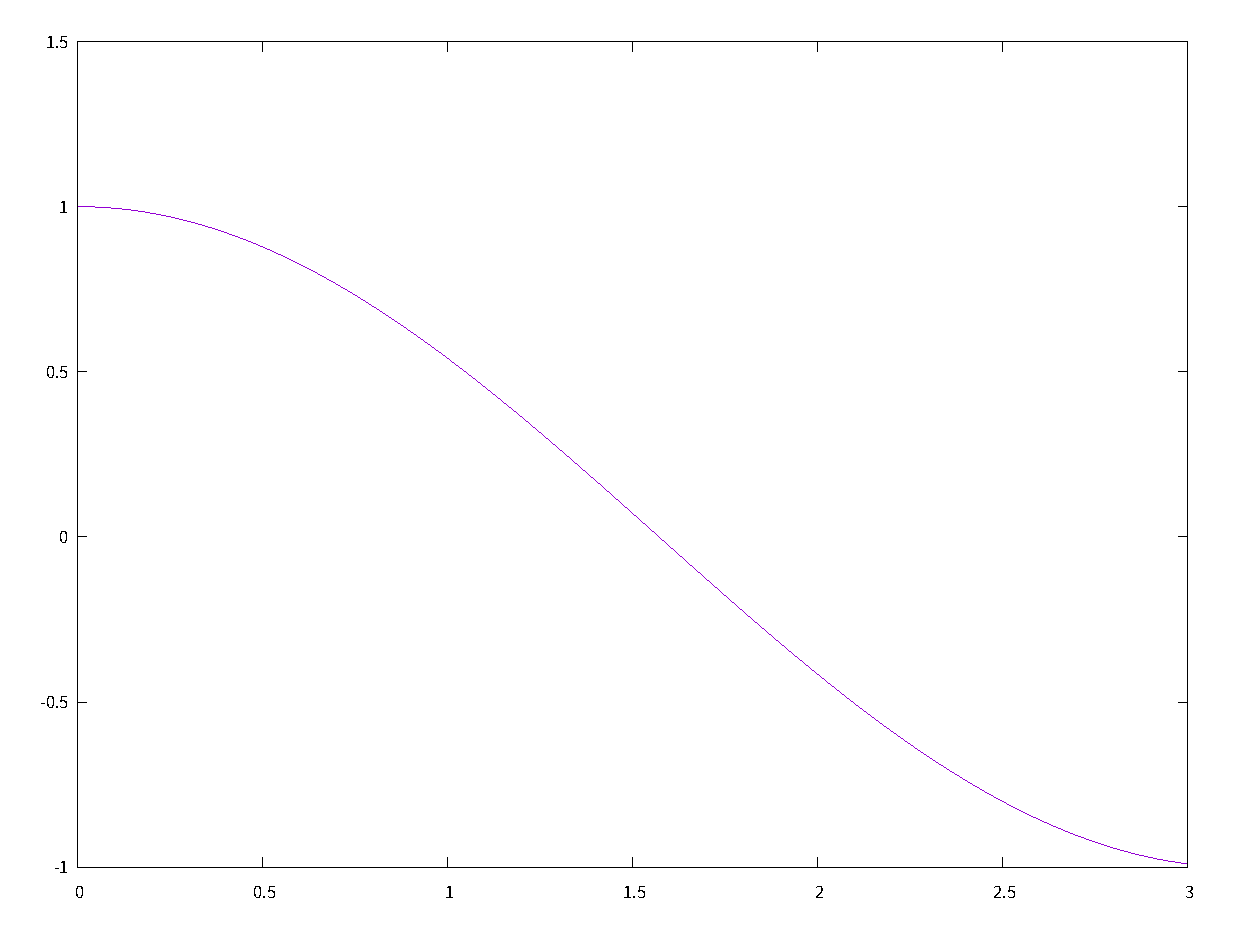
\includegraphics[width=0.4\textwidth]{pic/1-1.eps}
    \caption{The exact solution to (1).}
  \end{figure}
\end{frame}

\begin{frame}
  \frametitle{A sample stiff problem}
  The classical RK method goes to $\infty$ immediately.
  \begin{figure}
    \centering
    \includegraphics[width=0.2\textwidth]{pic/1-2.png}
    \caption{The numerical results given by the classical RK method.}
  \end{figure}
  
  The Gauss-Legendre RK methods give the following results.
  \begin{figure}[H]
    \centering
    \begin{minipage}[t]{0.32\linewidth}
        \centering
        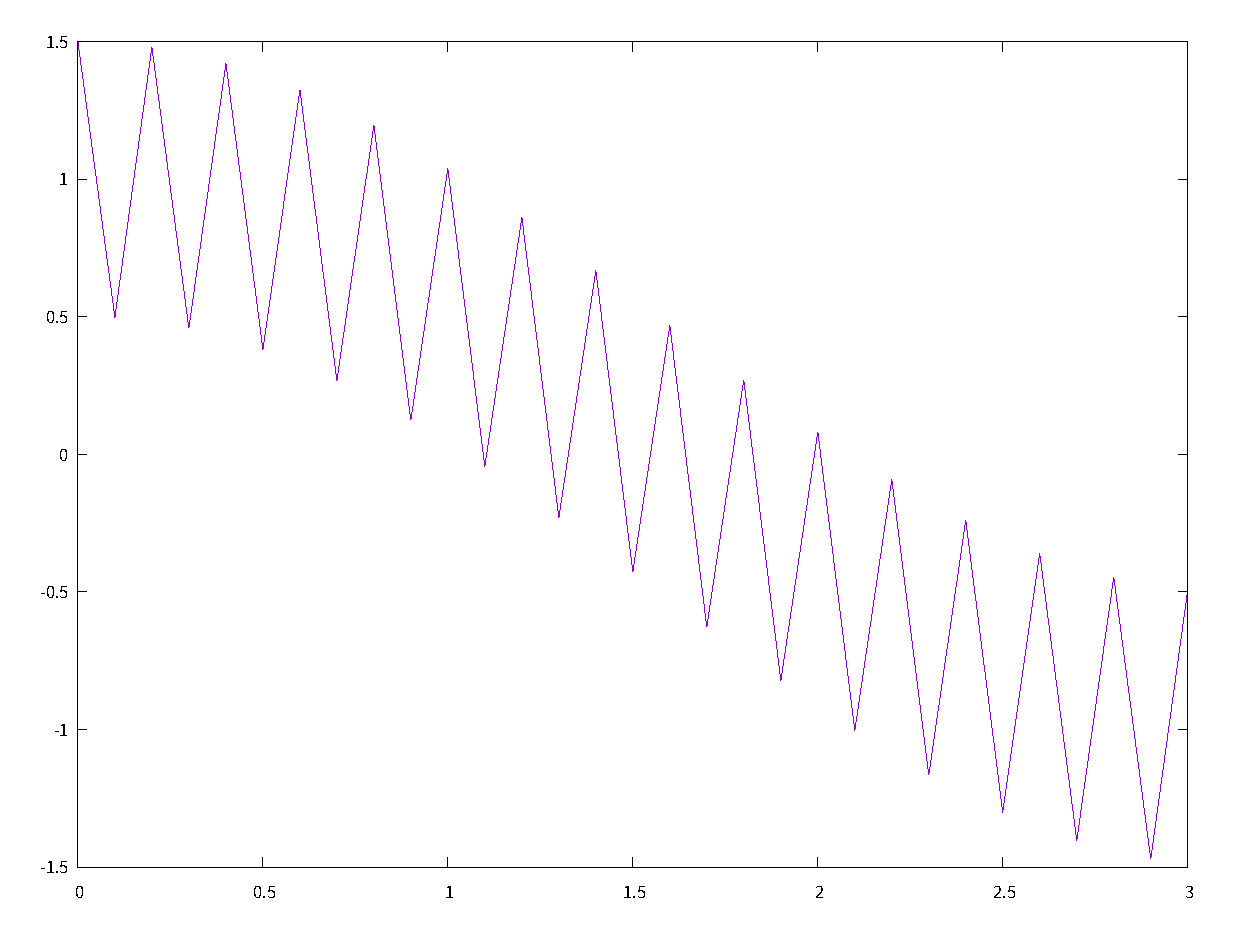
\includegraphics[width=0.95\linewidth]{pic/1-3.eps}
        \caption{$s=1$}
    \end{minipage}
    \begin{minipage}[t]{0.32\linewidth}
        \centering
        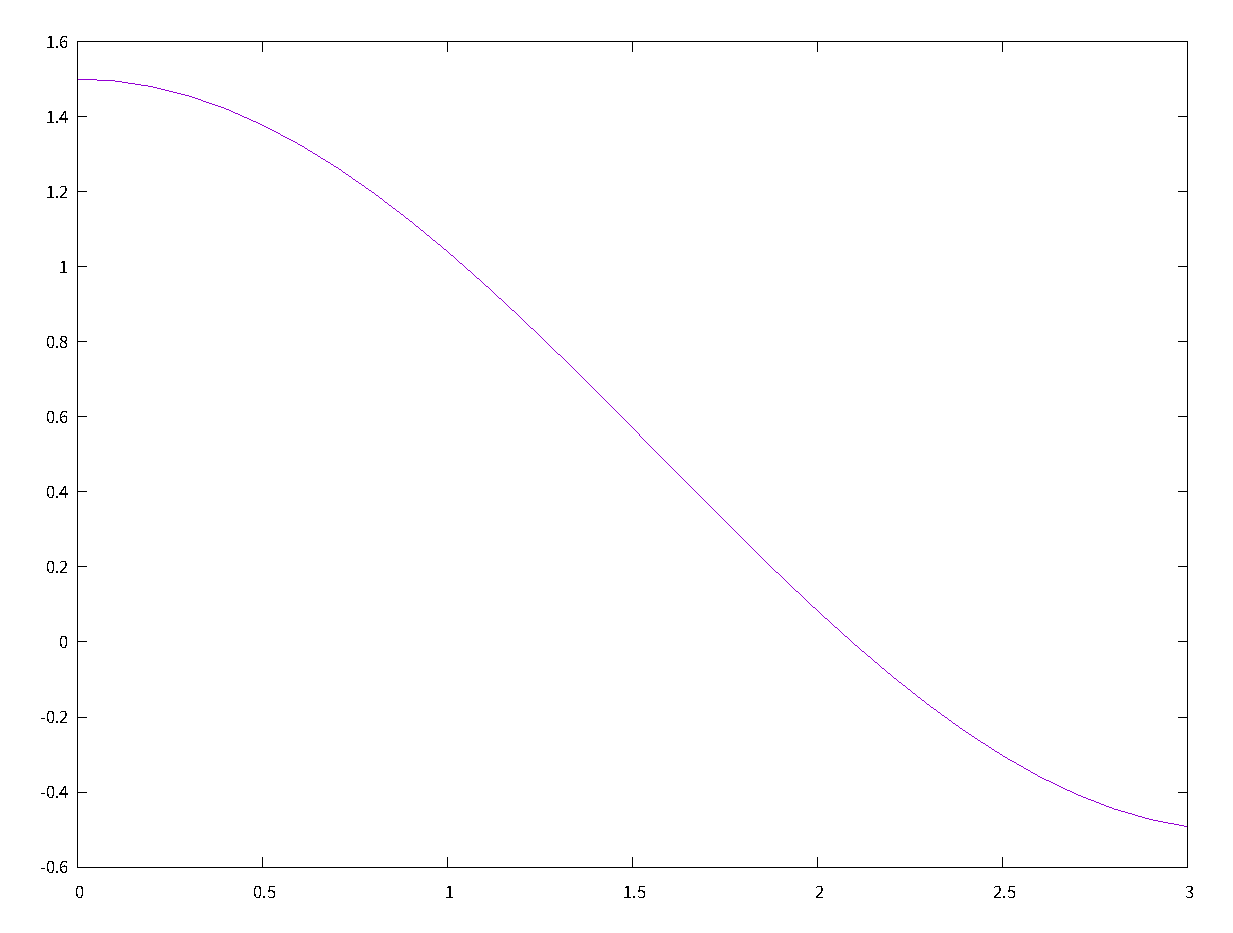
\includegraphics[width=0.95\linewidth]{pic/1-4.eps}
        \caption{$s=2$}
    \end{minipage}
    \begin{minipage}[t]{0.32\linewidth}
        \centering
        \includegraphics[width=0.95\linewidth]{pic/1-5.eps}
        \caption{$s=3$}
    \end{minipage}
  \end{figure}
\end{frame}

\begin{frame}
  \frametitle{A sample stiff problem}
  The Dormand-Prince method also performs badly. It used 903579 time steps to solve (1) with the tolerance $10^{-6}$.

  \vspace{1em}
  To solve (1), we need an L-stable method. The backward Euler method or the ESDIRK method in the textbook could be used, which have order 1 and 4 respectively.
\end{frame}

\begin{frame}
  \frametitle{A famous stiff problem - Van der Pol equation}

  The Van der Pol equation is
  \begin{equation}
    u''=\lambda (1-u^2)u'-u,\quad u(0)=2,\quad u'(0)=0,
  \end{equation}
  where $\lambda=1000$.

  \begin{figure}
    \centering
    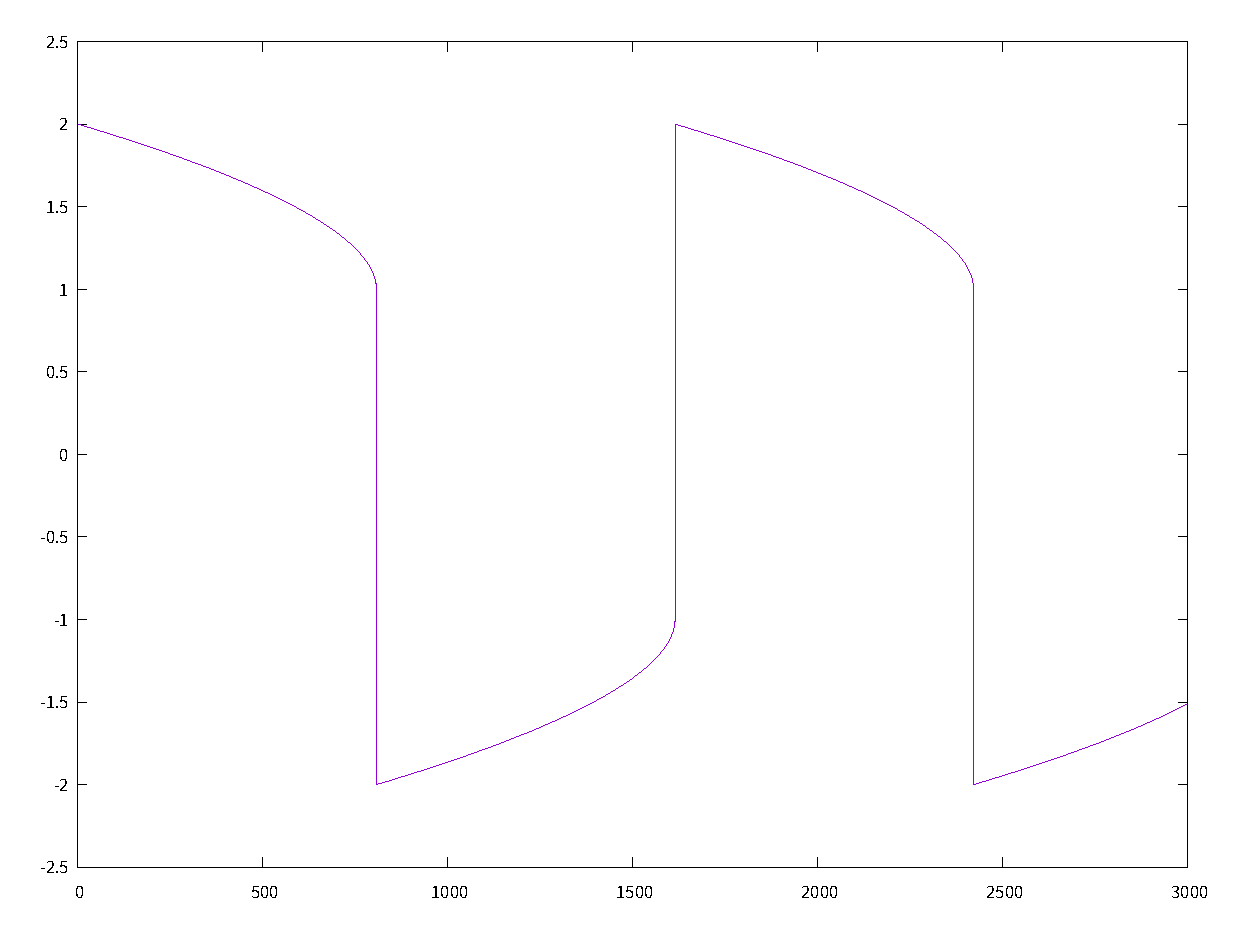
\includegraphics[width=0.4\textwidth]{pic/1-6.eps}
    \caption{The exact solution to (2).}
  \end{figure}

  No method in the assignment can solve the problem well!
\end{frame}

\section{An adaptive ESDIRK method}

\begin{frame}
  \frametitle{Introduction}

  Our motivation is to solve the Van der Pol's equation. Use Richardson extrapolation
  \begin{align*}
    \mathbf{U}^{n+\frac{1}{2}}&=\mathbf{U}^n+\frac{k}{2}\boldsymbol{\Phi}\left(\mathbf{U}^n,t_n;\frac{k}{2}\right),\\
    \tilde{\mathbf{U}}^{n+1}&=\mathbf{U}^{n+\frac{1}{2}}+\frac{k}{2}\boldsymbol{\Phi}\left(\mathbf{U}^{n+\frac{1}{2}},t_n+\frac{k}{2};\frac{k}{2}\right),\\
    \hat{\mathbf{U}}^{n+1}&=\tilde{\mathbf{U}}^{n+1}+\frac{1}{2^p-1}\left(\tilde{\mathbf{U}}^{n+1}-\mathbf{U}^{n+1}\right)
  \end{align*}
  to get $\hat{\mathbf{U}}^{n+1}$. The remaining steps are the same as the Formula 11.234.

\end{frame}

\begin{frame}
  \frametitle{Numericacl experiment}

  Use the adaptive ESDIRK method to solve the Van der Pol equation. The following table shows the steps and CPU times it takes.
  \begin{table}[H]
    \centering
    \begin{tabular}{c|cccc}
      Tolerance & $10^{-4}$ & $10^{-6}$ & $10^{-8}$ & $10^{-10}$ \\ \hline
      Steps & 376 & 638 & 1273 & 3382   \\
      CPU Time(s) & 0.375  & 0.296 & 0.161 & 0.254 
    \end{tabular}
  \end{table}
  
  The following figure is the solution with the tolerance $10^{-4}$.

  \begin{figure}
    \centering
    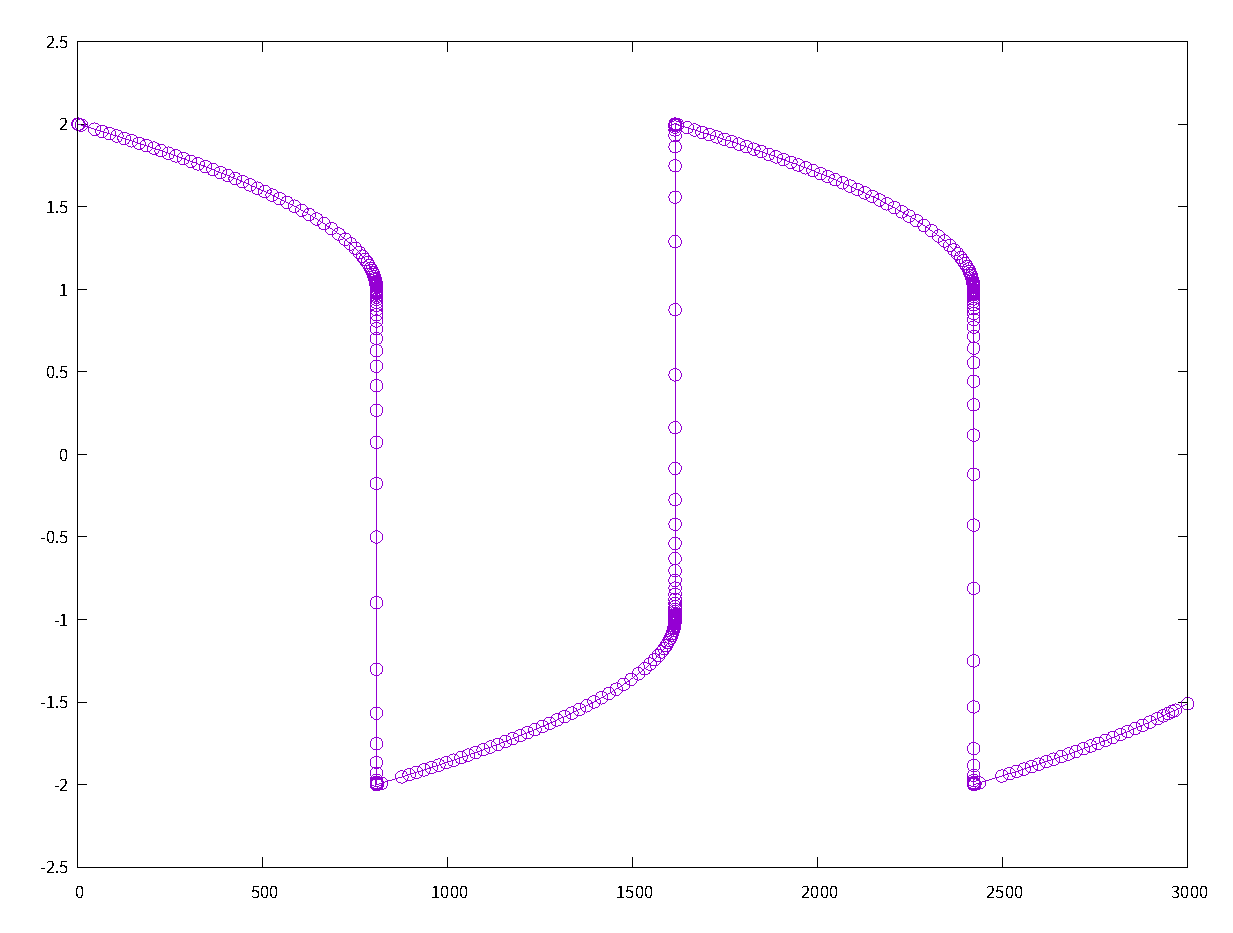
\includegraphics[width=0.4\textwidth]{pic/2-1.eps}
  \end{figure}

\end{frame}

\section{The Radau-IIA methods}

\begin{frame}
  \frametitle{A review of Gauss-Legendre methods}

  Recall that how we construct the $s$-stages Gauss-Legendre method.

  \pause

  \vspace{1em}
  Let $c_1,...,c_s$ be the roots of $P_s(x)$, where $P_s$ is a polynomial of degree $s$ and has distinct roots (see the textbook). Then we let
  \begin{align*}
    a_{ij}&=\int_0^{c_i} l_j(x)\text{d} x\\
    b_j&=\int_0^1 l_j(x)\text{d} x
  \end{align*}
  where $l_j$ is the elementary Lagrange interpolation polynomial.

  \vspace{1em}
  It constructs a $s$-stages, $(2s)$th-order collocation method, which is A-stable and B-stable but not L-stable. The order could be arbitrary high without extra artificial work.

  \vspace{1em}
  We can derive adaptive Gauss-Legendre methods immediately with Richardson extrapolation. 
\end{frame}

\begin{frame}
  \frametitle{Solving the stiff problem with adaptive Gauss-Legendre methods}
  Adaptive Gauss-Legendre methods perform well in the Van der Pol equation. The solution with the tolerance $10^{-4}$ are shown as follows.

\begin{figure}[H]
  \centering
  \begin{minipage}[t]{0.32\linewidth}
      \centering
      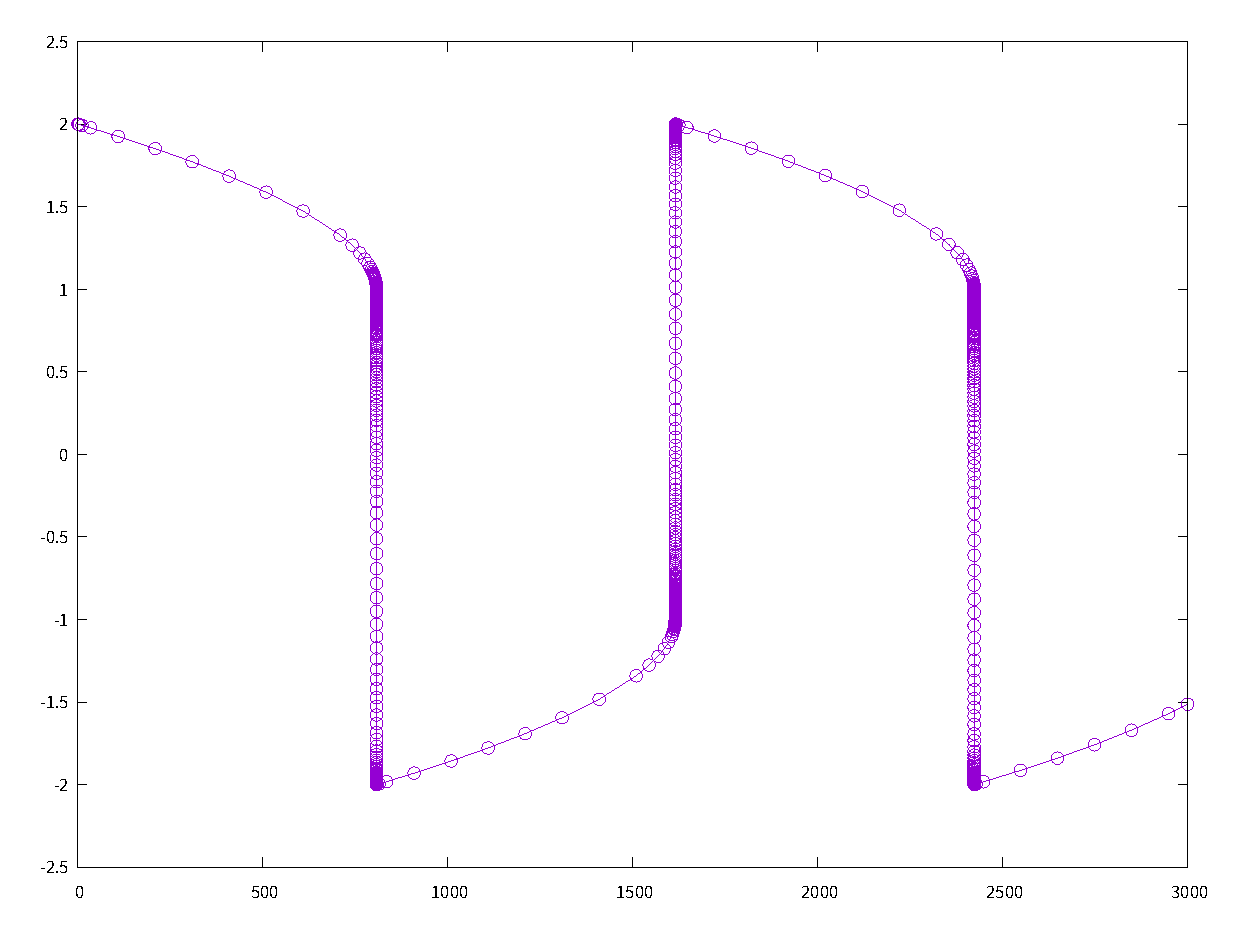
\includegraphics[width=0.95\linewidth]{pic/7-4.eps}
      \vspace{-1em}
      \caption{\small $s=1$, $n=918$}
  \end{minipage}
  \begin{minipage}[t]{0.32\linewidth}
      \centering
      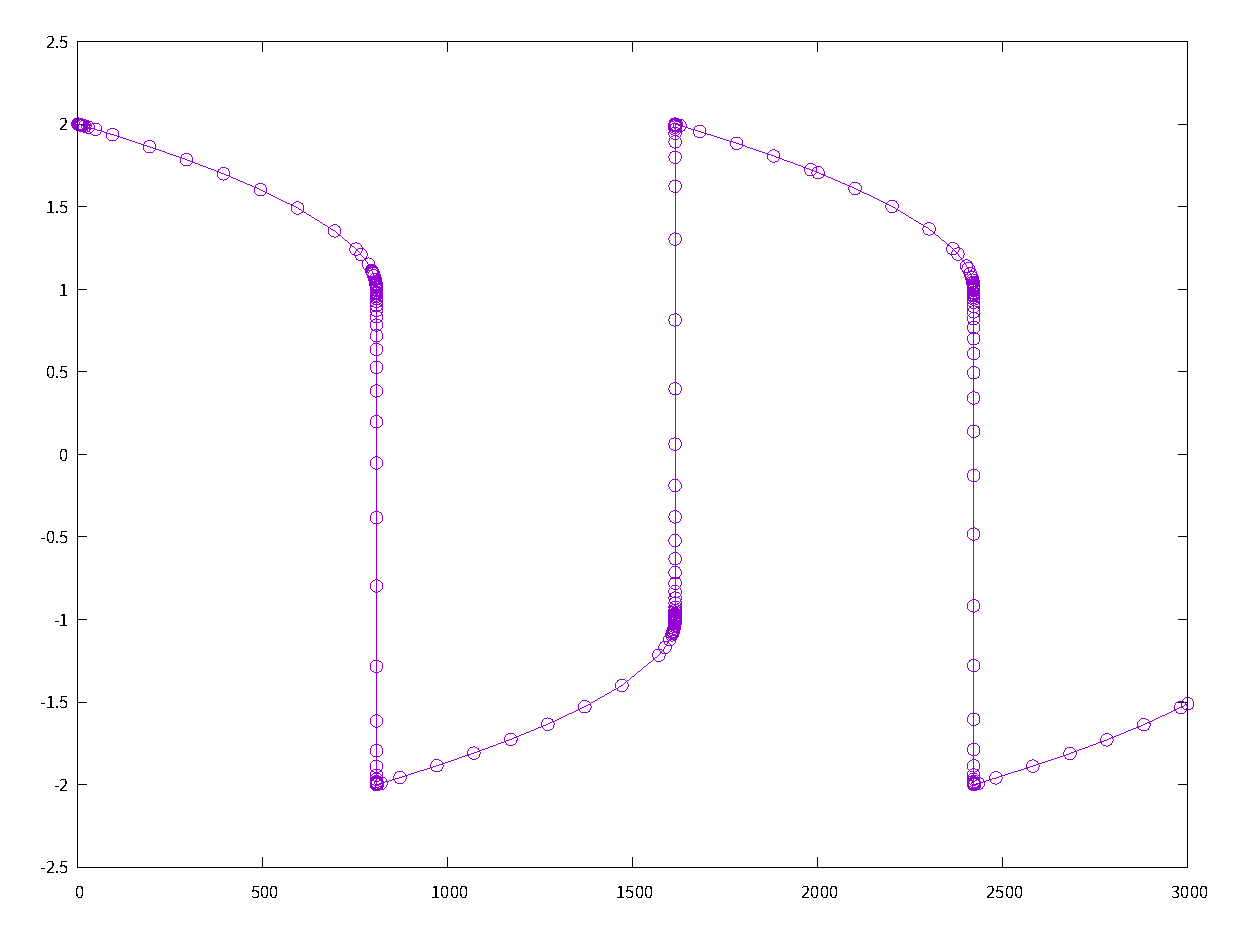
\includegraphics[width=0.95\linewidth]{pic/7-5.eps}
      \vspace{-1em}
      \caption{\small $s=2$, $n=269$}
  \end{minipage}
  \begin{minipage}[t]{0.32\linewidth}
      \centering
      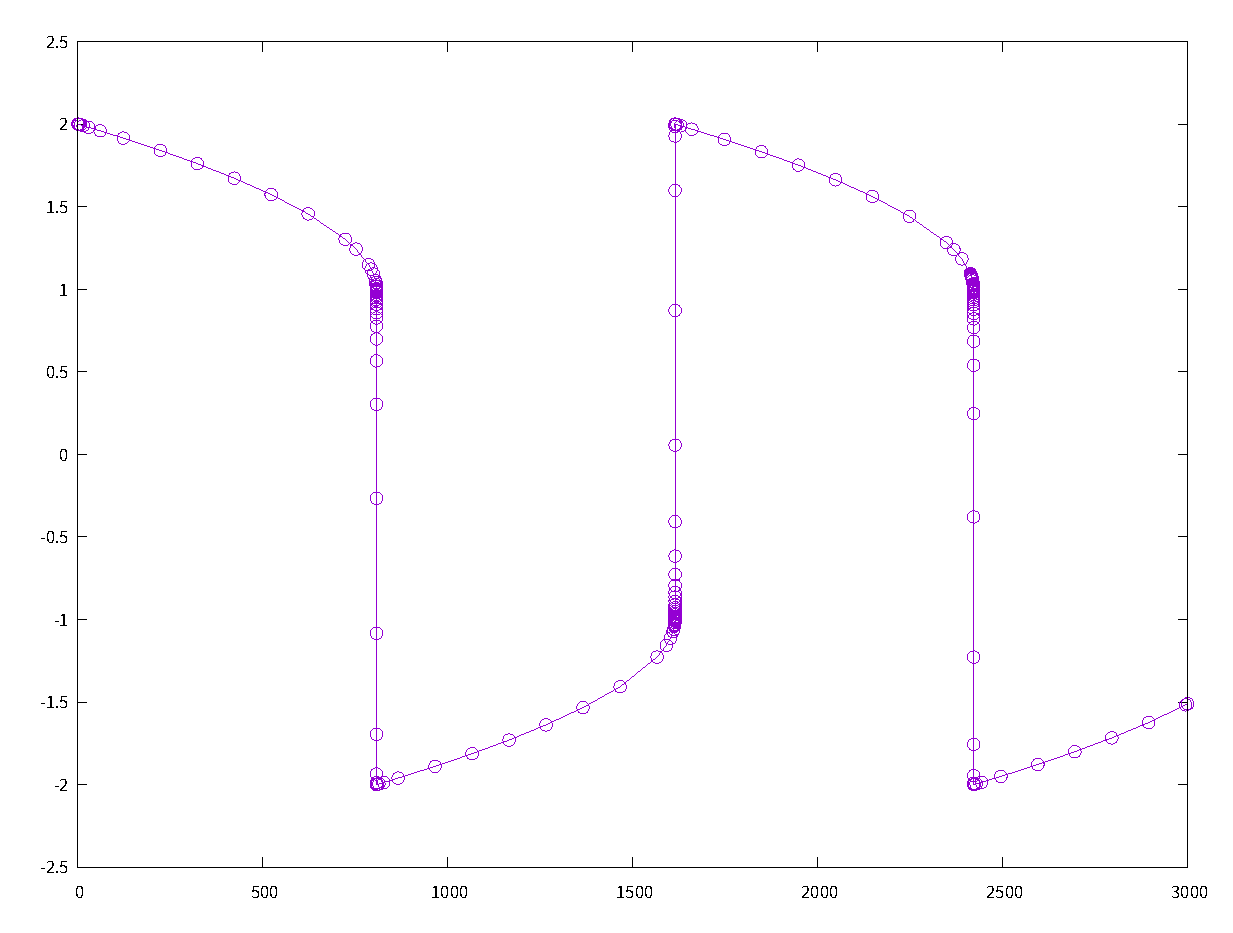
\includegraphics[width=0.95\linewidth]{pic/7-6.eps}
      \vspace{-1em}
      \caption{\small $s=3$, $n=207$}
  \end{minipage}
\end{figure}

\pause

However, the adaptive $3$-stages Gauss-Legendre method takes $5.46$s to solve the problem (1) with the tolerance $10^{-13}$. The adaptive ESDIRK method also takes $3.7$s. We think they are too slow.

\end{frame}

\begin{frame}
  \frametitle{Constructing Radau-IIA methods}

  The motivation is to construct a high-order, adaptive and L-stable method.
  \pause

  Suppose the polynomial
  \begin{equation*}
    Q_s(x)=\frac{\text{d}^{s-1}}{\text{d}x^{s-1}} x^{s-1}(x-1)^s.
  \end{equation*}

  It can be proved that $Q_s$ has $s$ distinct roots located in $(0,1]$. Let $c_1,...,c_s$ to be the roots of $Q(s)$ and then derive a collocation method.

  \vspace{1em}
  The $s$-stages Radau-IIA method has $(2s-1)$th-order and is L-stable. And also we can derive adaptive Radau-IIA methods.
\end{frame}

\begin{frame}
  \frametitle{Solving stiff problems with adaptive Radau-IIA methods}
  Adaptive Radau-IIA methods perform well in the Van der Pol equation. The solution with the tolerance $10^{-4}$ are shown as follows.

\begin{figure}[H]
  \centering
  \begin{minipage}[t]{0.32\linewidth}
      \centering
      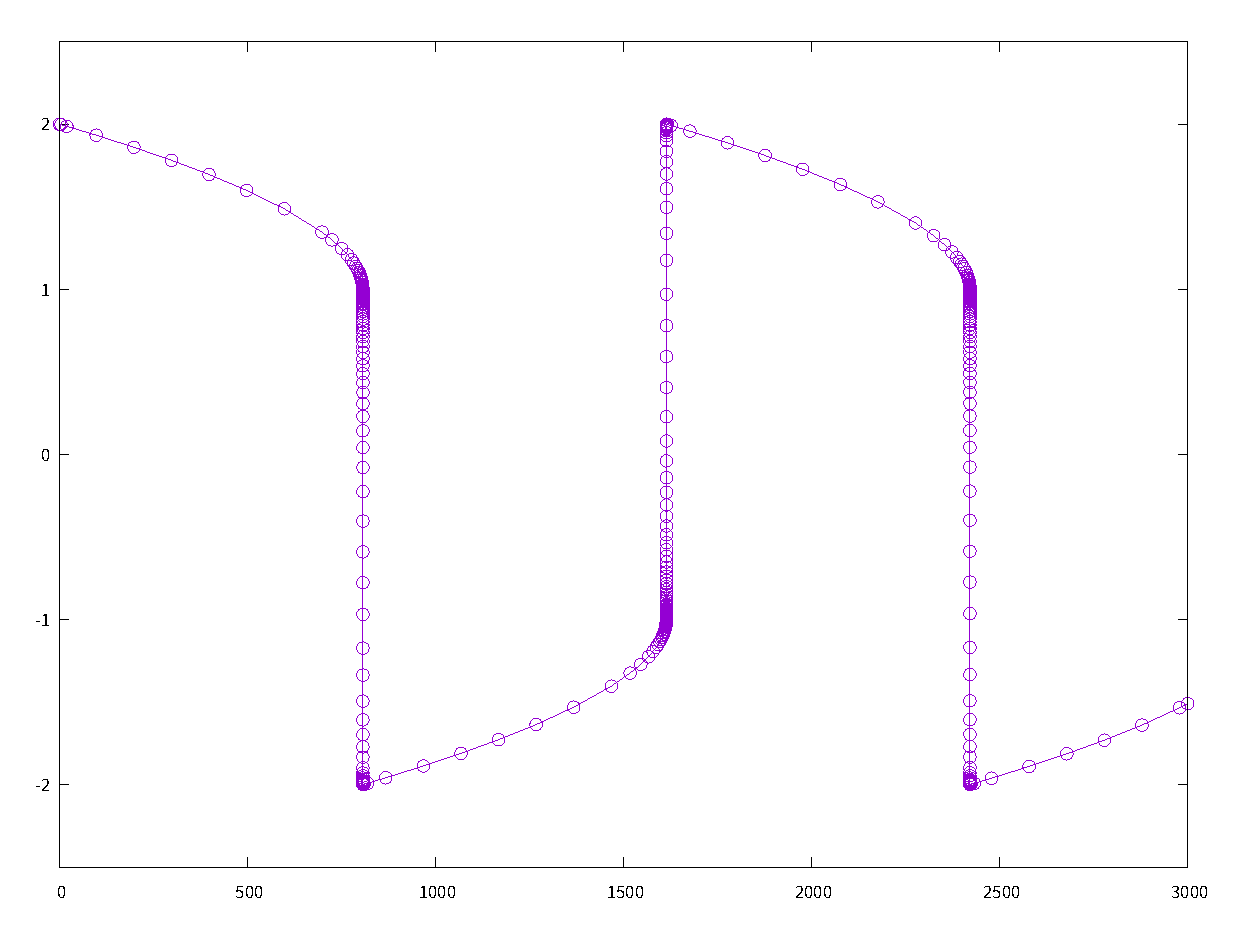
\includegraphics[width=0.95\linewidth]{pic/9-6.eps}
      \vspace{-1em}
      \caption{\small $s=2$, $n=421$}
  \end{minipage}
  \begin{minipage}[t]{0.32\linewidth}
      \centering
      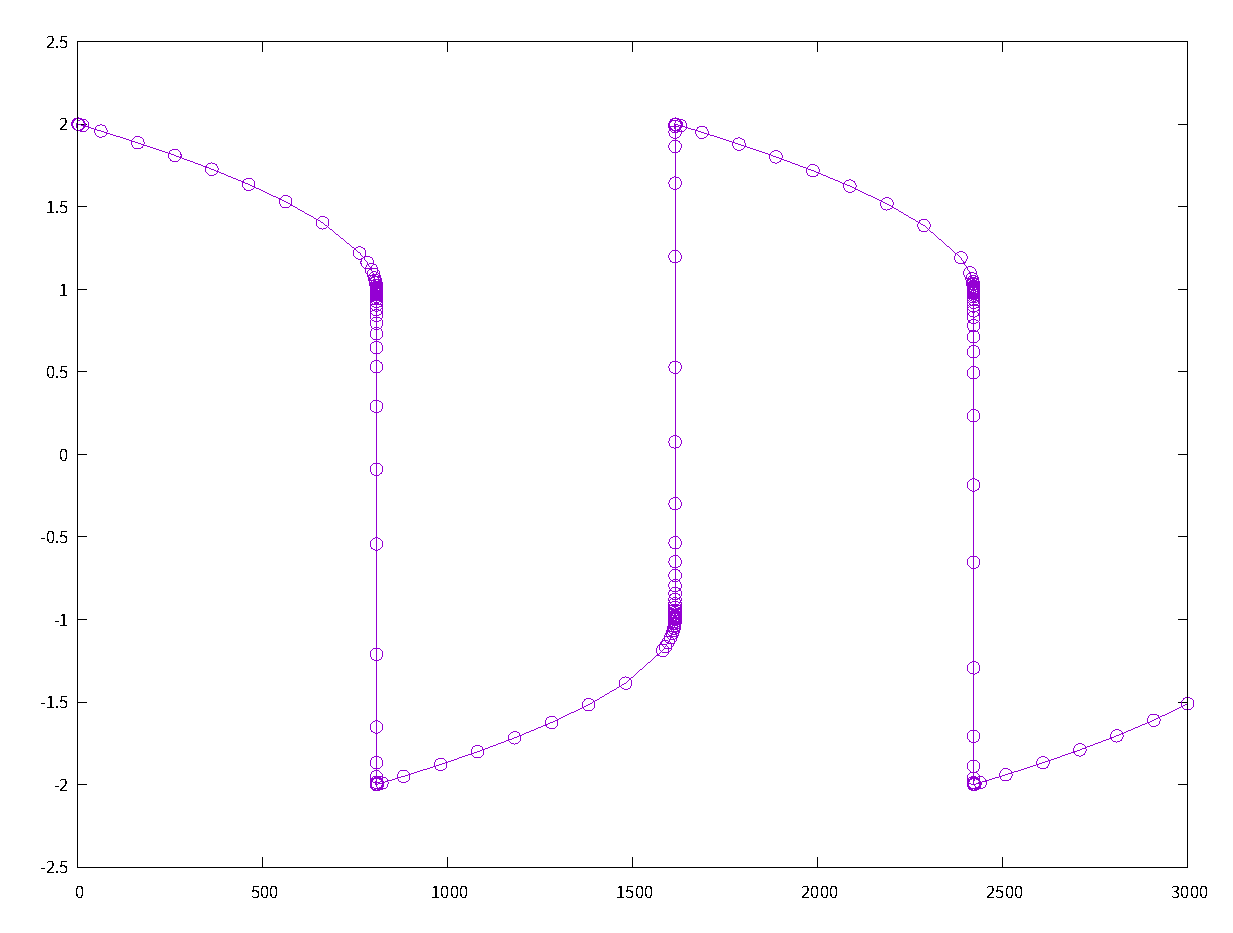
\includegraphics[width=0.95\linewidth]{pic/9-7.eps}
      \vspace{-1em}
      \caption{\small $s=3$, $n=200$}
  \end{minipage}
  \begin{minipage}[t]{0.32\linewidth}
      \centering
      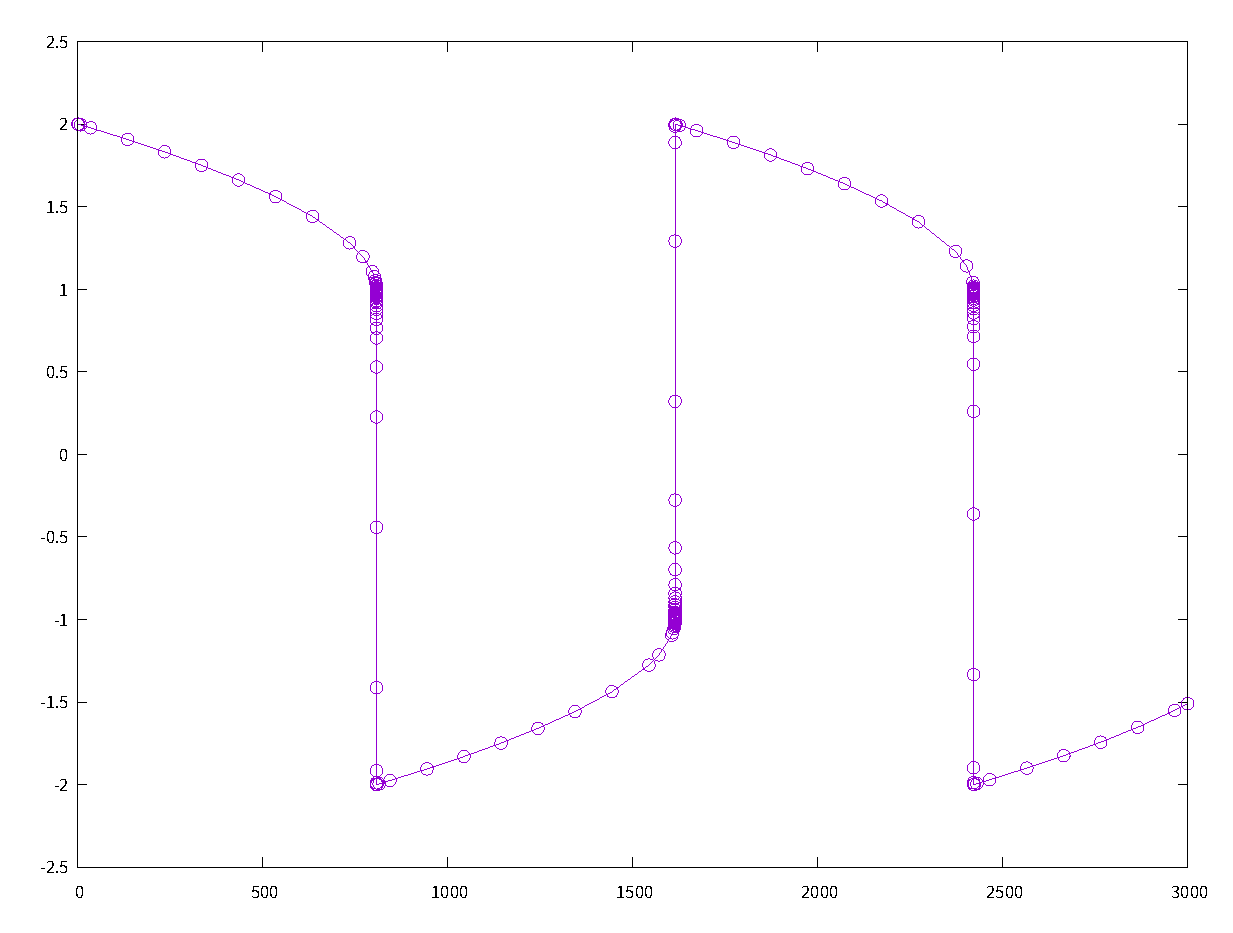
\includegraphics[width=0.95\linewidth]{pic/9-8.eps}
      \vspace{-1em}
      \caption{\small $s=4$, $n=170$}
  \end{minipage}
\end{figure}

\end{frame}

\begin{frame}
  \frametitle{Solving stiff problems with adaptive Radau-IIA methods}

Use the A-RIIARK$3$ method to solve the problem (1), comparing with the A-GLRK$3$ method as the following figures.

\begin{figure}[H]
  \centering
  \begin{minipage}[t]{0.4\linewidth}
      \centering
      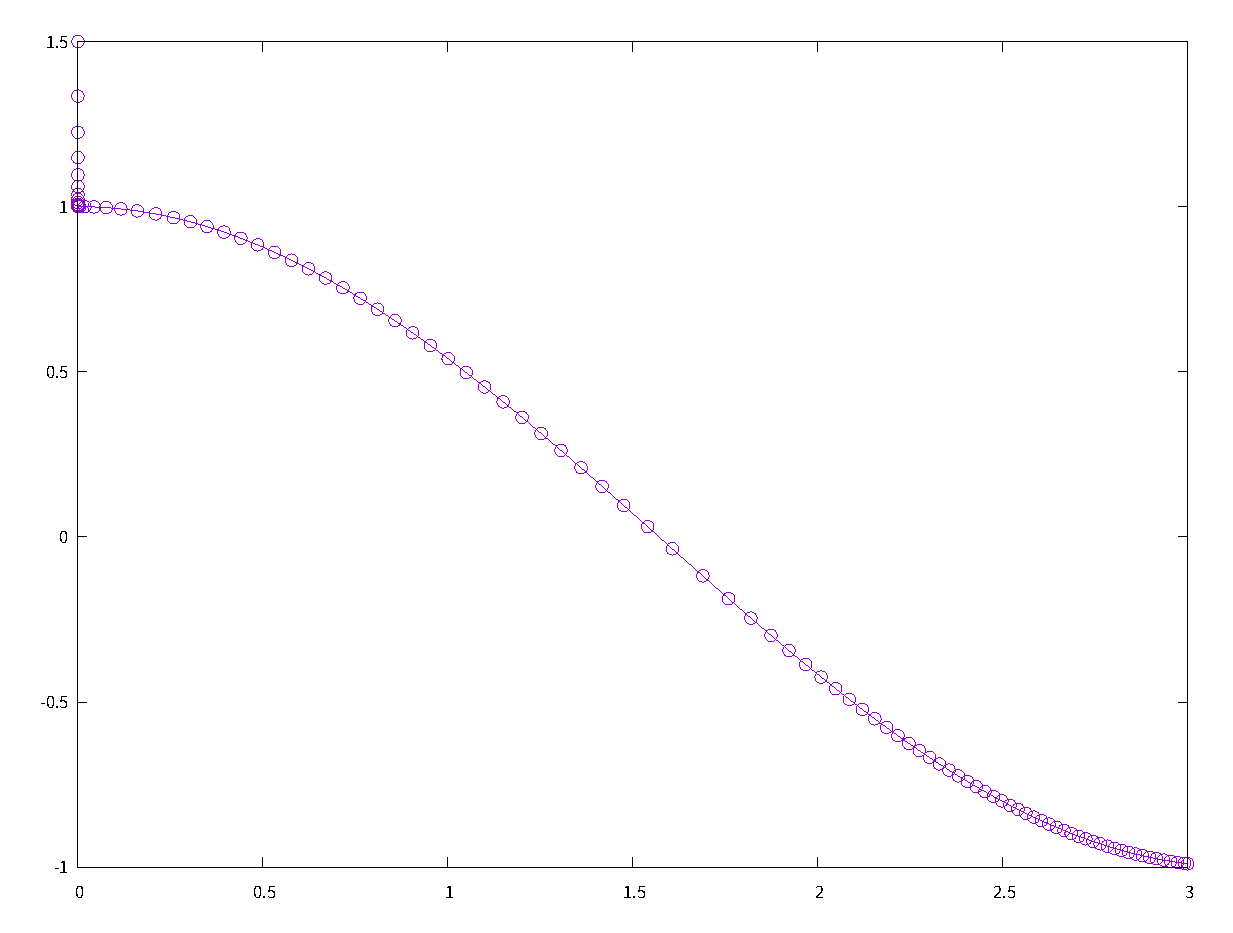
\includegraphics[width=0.9\linewidth]{pic/10-2.eps}
      \caption{\small A-GLRK$3$, $n=109$, $5.46$s}
  \end{minipage}
  \hspace{2em}
  \begin{minipage}[t]{0.4\linewidth}
      \centering
      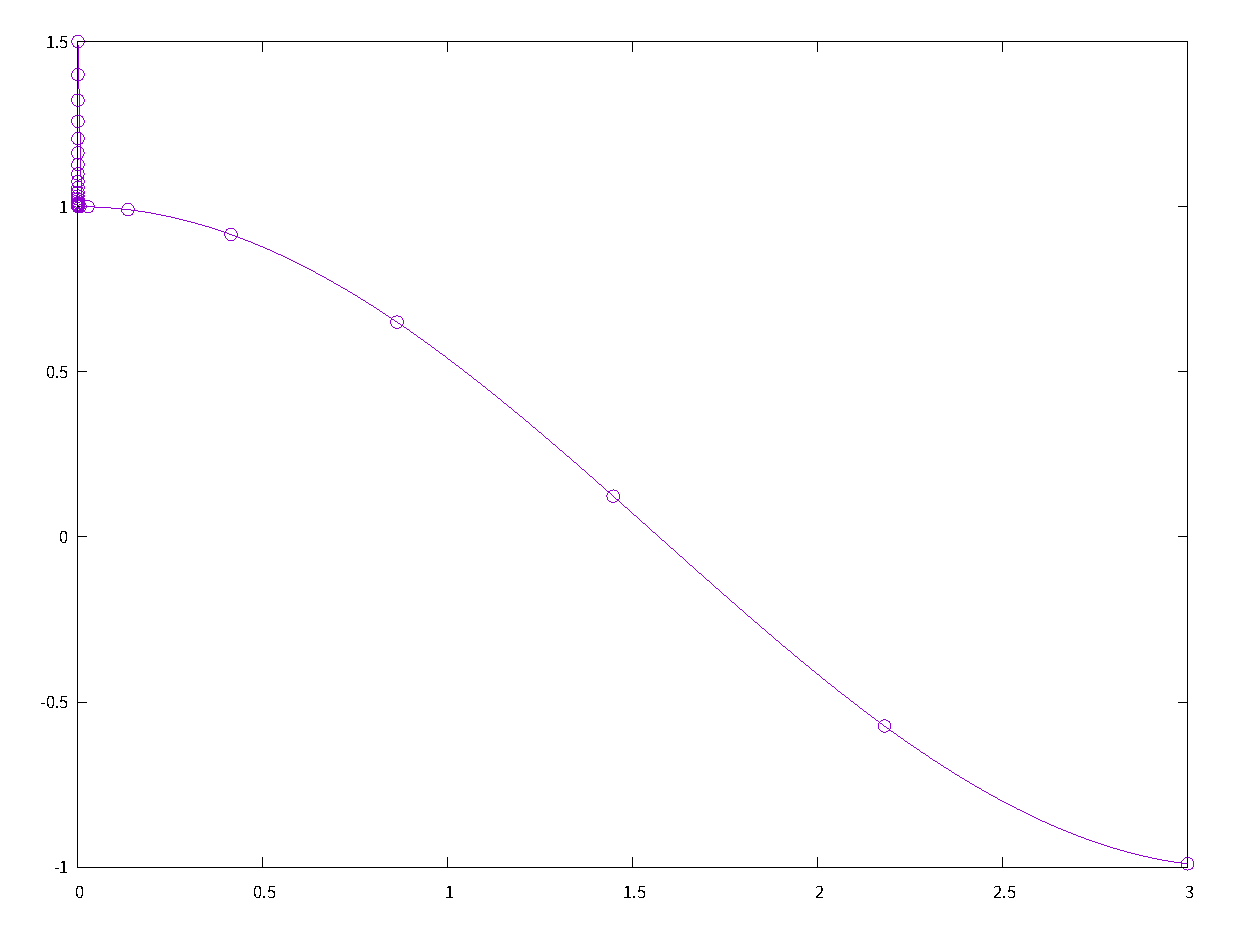
\includegraphics[width=0.9\linewidth]{pic/10-3.eps}
      \caption{\small A-RIIARK$3$, $n=43$, $0.769$s}
  \end{minipage}
\end{figure}

\end{frame}

\begin{frame}
    \frametitle{Thanks}
    \centering
    \Large Thaks for Your Attention!
\end{frame}

\end{document}
